% Build: tectonic report.tex
\documentclass[11pt,a4paper]{article}

\usepackage[vietnamese]{babel}
\usepackage{fontspec}
\setmainfont{BeVietnamPro}[Path=fonts/, Extension=.ttf,
  UprightFont=*-Regular, BoldFont=*-Bold, ItalicFont=*-Italic]
\setsansfont{BeVietnamPro}[Path=fonts/, Extension=.ttf,
  UprightFont=*-Regular, BoldFont=*-Bold, ItalicFont=*-Italic]
\setmonofont{Menlo}[Scale=0.82]

\usepackage[margin=2.5cm]{geometry}
\usepackage{graphicx}
\usepackage{booktabs}
\usepackage{tabularx}
\usepackage{array}
\usepackage{xcolor}
\usepackage{listings}
\usepackage{enumitem}
\usepackage{caption}
\usepackage{float}
\usepackage{amsmath,amssymb}
\emergencystretch=3em
\newcommand{\yes}{$\checkmark$}
\usepackage{tikz}
\usetikzlibrary{positioning,arrows.meta,fit}
\usepackage{titlesec}
\usepackage{fancyhdr}
\usepackage[hidelinks]{hyperref}

\definecolor{ink}{HTML}{142E49}
\definecolor{copper}{HTML}{CA6B3E}
\definecolor{copperdark}{HTML}{A64C27}
\definecolor{teal}{HTML}{1F5568}
\definecolor{muted}{HTML}{5F686F}
\definecolor{paper}{HTML}{F6F3EE}
\definecolor{line}{HTML}{E0DBD0}

\newcommand{\TODO}[1]{\textcolor{red}{[#1]}}
\newcommand{\code}[1]{\texttt{#1}}

\titleformat{\section}{\sffamily\Large\bfseries\color{ink}}{\thesection}{0.8em}{}
\titleformat{\subsection}{\sffamily\large\bfseries\color{ink}}{\thesubsection}{0.8em}{}
\titleformat{\subsubsection}{\sffamily\normalsize\bfseries\color{ink}}{\thesubsubsection}{0.8em}{}

\lstset{
  basicstyle=\ttfamily\small,
  keywordstyle=\color{teal}\bfseries,
  commentstyle=\color{muted}\itshape,
  stringstyle=\color{copperdark},
  backgroundcolor=\color{paper},
  frame=single, rulecolor=\color{line},
  framesep=6pt, xleftmargin=6pt, xrightmargin=6pt,
  breaklines=true, columns=fullflexible, keepspaces=true,
  showstringspaces=false
}
\lstdefinelanguage{psql}[]{SQL}{
  morekeywords={rollup,cube,grouping,sets,materialized,refresh,conflict,excluded,returning,distinct,lag,over,partition,rank,coalesce},
  sensitive=false
}

\setlist{itemsep=2pt, topsep=4pt}
\captionsetup{font=small, labelfont={bf,color=ink}}
\setlength{\parskip}{4pt}
\renewcommand{\arraystretch}{1.18}

\pagestyle{fancy}
\fancyhf{}
\fancyhead[L]{\small\sffamily\color{muted}CO4031 | Kho dữ liệu và Hệ hỗ trợ quyết định}
\fancyhead[R]{\small\sffamily\color{muted}CoinSight}
\fancyfoot[C]{\small\thepage}
\renewcommand{\headrulewidth}{0.4pt}

\begin{document}

% ---------------------------------------------------------------- bìa
\begin{titlepage}
\centering
{\sffamily\large ĐẠI HỌC QUỐC GIA THÀNH PHỐ HỒ CHÍ MINH\\
TRƯỜNG ĐẠI HỌC BÁCH KHOA\\
KHOA KHOA HỌC VÀ KỸ THUẬT MÁY TÍNH\par}
\vspace{1.0cm}

\includegraphics[width=3.4cm]{figures/bk.png}\par
\vspace{1.0cm}
{\sffamily\large KHO DỮ LIỆU VÀ HỆ HỖ TRỢ QUYẾT ĐỊNH (CO4031)\par}
\vspace{0.6cm}
{\sffamily\Large\bfseries BÁO CÁO BÀI TẬP LỚN\par}
\vspace{0.5cm}
{\sffamily\huge\bfseries\color{ink}\raisebox{-0.22em}{
\includegraphics[height=1.15em]{figures/logo.pdf}}\ CoinSight\par}
\vspace{0.2cm}
{\sffamily\large\color{muted} Kho dữ liệu nến giá crypto và hệ hỗ trợ quyết định\par}
\vspace{1.4cm}
\begin{tabular}{ll}
Giảng viên hướng dẫn: & ThS. Đỗ Thanh Thái \\
Nhóm: & 7 \quad Lớp: L02 \\[6pt]
\end{tabular}

\begin{tabular}{lll}
\toprule
\textbf{Họ và tên} & \textbf{MSSV} & \textbf{Vai trò} \\
\midrule
Lê Chí Đại & 2310621 & Luồng trực tiếp, API, giao diện, agent \\
Hà Bảo Nhi & 2312496 & Thiết kế kho, ETL, chất lượng dữ liệu, OLAP \\
Đào Quang Dương & 2310579 & DSS: mô hình dự báo và đánh giá \\
\bottomrule
\end{tabular}

\vspace{1.0cm}
\begin{tabular}{ll}
Video thuyết trình: & \TODO{link YouTube unlisted / Google Drive} \\
Mã nguồn: & \url{https://github.com/caoTayTang/CoinSight} \\
\end{tabular}

\vfill
{\sffamily Thành phố Hồ Chí Minh, tháng 11 năm 2026\par}
\end{titlepage}

\tableofcontents
\newpage

% ---------------------------------------------------------------- 1
\section{Giới thiệu}

\subsection{Bối cảnh và bài toán}
Thị trường crypto giao dịch liên tục 24/7, mỗi coin sinh ra hàng nghìn nến giá mỗi năm.
Người theo dõi thị trường hay hỏi hai kiểu câu. Kiểu thứ nhất hỏi về chuyện đã xảy ra:
quý vừa rồi nhóm coin nào tăng mạnh nhất, nhóm nào biến động nhiều nhất, phiên châu Á, châu
Âu hay châu Mỹ sôi động hơn, coin nào vào top tăng giảm mỗi quý. Kiểu thứ hai hỏi về chuyện
sắp xảy ra: ngày mai BTC có tăng không, và quan trọng hơn, có nên tin vào con số dự báo đó không.

Dữ liệu thô từ sàn (file ZIP theo ngày/tháng, luồng WebSocket) không trả lời được trực tiếp
các câu hỏi này: dữ liệu rải rác nhiều file, có thể trùng, thiếu, sai, và không có sẵn
các chiều phân tích như quý, nhóm coin hay phiên giao dịch. Nhóm xây dựng \textbf{CoinSight}:
một kho dữ liệu (data warehouse) tích hợp lịch sử nến giá của 20 coin từ Binance, các
mart OLAP trả lời nhóm câu hỏi thứ nhất, và một thành phần hỗ trợ quyết định (DSS) trả
lời nhóm câu hỏi thứ hai.

\subsection{Mục tiêu}
\begin{itemize}
  \item Thiết kế kho dữ liệu đa chiều theo phương pháp Kimball, với grain rõ ràng cho từng bảng fact.
  \item Xây dựng quy trình ETL có kiểm tra chất lượng, nạp lại an toàn (idempotent) và truy vết được về file nguồn.
  \item Xây dựng các mart OLAP bằng \code{ROLLUP}, \code{CUBE}, \code{GROUPING SETS} phục vụ roll-up, drill-down, slice, dice.
  \item Hiện thực backend (PostgreSQL, ETL, API) và frontend (dashboard, giao diện hỏi đáp).
  \item Xây dựng DSS dự báo hướng giá dựa trên kho, có cơ chế từ chối khi mô hình không tốt hơn baseline.
  \item Đánh giá kết quả, nêu rõ hạn chế.
\end{itemize}

\subsection{Phạm vi}
Nguồn dữ liệu là Binance Spot, cặp giao dịch với USDT. Kho lưu nến ngày và nến giờ cho
20 coin; dữ liệu lịch sử lấy từ Binance Public Data (\url{https://data.binance.vision}).
Giá và khối lượng tính theo USDT. Hệ thống chỉ đọc dữ liệu thị trường và không đặt lệnh
giao dịch thật.

\subsection{Đối chiếu chuẩn đầu ra}
\begin{table}[H]
\centering\small
\begin{tabularx}{\linewidth}{lX}
\toprule
\textbf{Chuẩn đầu ra} & \textbf{Nội dung tương ứng trong báo cáo} \\
\midrule
L.O.1.1--1.3 & Mục 1, 2: khái niệm DW/DSS, vai trò của kho trong DSS, ví dụ thực tế là CoinSight \\
L.O.2.1--2.3 & Mục 3--6: quy trình thiết kế Kimball, các vấn đề grain, SCD, khóa; hiện thực kho và ETL \\
L.O.3.1--3.3 & Mục 7: DSS theo mô hình ra quyết định của Simon, mô hình hóa bài toán dự báo \\
L.O.4.1--4.2 & Mục 7, 8: thiết kế, hiện thực, đánh giá DSS dự báo hướng giá \\
\bottomrule
\end{tabularx}
\end{table}

% ---------------------------------------------------------------- 2
\section{Cơ sở lý thuyết}

\subsection{Kho dữ liệu}
Theo Inmon, kho dữ liệu là tập dữ liệu \emph{hướng chủ đề, tích hợp, ổn định và theo thời gian}
phục vụ ra quyết định. Trong CoinSight, chủ đề là giá và khối lượng giao dịch của coin.
Dữ liệu lịch sử (ZIP) và dữ liệu trực tiếp (WebSocket) dùng chung \code{dim\_asset} và
\code{dim\_date}, mọi giá quy về USDT, nên hai nguồn được tích hợp. Nến đã đóng không bị sửa,
và nạp lại cùng một file không làm đổi dữ liệu. Mỗi dòng fact gắn với một ngày hoặc một giờ
UTC, lịch sử không bị ghi đè khi có dữ liệu mới.

\subsection{Mô hình đa chiều}
Nhóm theo phương pháp bốn bước của Kimball: (1) chọn quy trình nghiệp vụ, (2) khai báo grain,
(3) xác định dimension, (4) xác định fact. Khi nhiều bảng fact dùng chung các dimension
(conformed dimension), lược đồ là \emph{galaxy schema} (fact constellation).

\subsection{OLAP}
Các phép OLAP dùng trong dự án: \emph{roll-up} (tháng $\rightarrow$ quý $\rightarrow$ năm),
\emph{drill-down} (ngược lại), \emph{slice} (cố định một chiều, ví dụ một quý),
\emph{dice} (lọc nhiều chiều), \emph{pivot}. PostgreSQL hỗ trợ trực tiếp \code{ROLLUP},
\code{CUBE}, \code{GROUPING SETS}; nhóm tính sẵn các tổng hợp nặng thành materialized view (ROLAP).

\subsection{Hệ hỗ trợ quyết định}
DSS theo Turban gồm ba thành phần: quản lý dữ liệu, quản lý mô hình và giao diện người dùng.
Quá trình ra quyết định theo Simon gồm ba pha: \emph{intelligence} (nhận diện vấn đề),
\emph{design} (xây dựng và đánh giá phương án), \emph{choice} (chọn phương án). Trong CoinSight,
kho dữ liệu là thành phần quản lý dữ liệu; mô hình dự báo là thành phần quản lý mô hình;
dashboard và agent hỏi đáp là giao diện.

% ---------------------------------------------------------------- 3
\section{Kiến trúc hệ thống}

Hệ thống có hai luồng vào cùng một kho, theo kiến trúc Lambda: luồng batch nạp lịch sử
chính xác, luồng trực tiếp cho dữ liệu mới nhất với độ trễ thấp.

\begin{figure}[H]
\centering
\begin{tikzpicture}[
  node distance=5mm and 7mm,
  box/.style={draw=line, fill=white, rounded corners=2pt, font=\sffamily\scriptsize,
    align=center, minimum height=8mm, text width=20mm},
  store/.style={box, fill=paper, draw=teal},
  arr/.style={-{Stealth[length=2mm]}, color=muted}]
\node[box] (zip) {Binance ZIP\\nến 1d, 1h};
\node[box, right=of zip] (stg) {Staging\\COPY};
\node[box, right=of stg] (dq) {Kiểm tra\\12 rule};
\node[store, right=of dq] (dw) {Kho \code{dw}\\fact + dim};
\node[store, right=of dw] (mart) {Mart OLAP\\\code{mart}};
\node[box, below=9mm of zip] (ws) {Binance WS\\nến 1m};
\node[box, right=of ws] (kafka) {Kafka};
\node[box, right=of kafka] (spark) {Spark\\Streaming};
\node[store, right=of spark] (live) {Fact trực tiếp};
\node[box, right=of live] (api) {FastAPI\\REST + WS};
\node[box, above=9mm of dw] (dss) {DSS\\mô hình dự báo};
\node[box, above=9mm of mart] (ui) {Dashboard\\Agent hỏi đáp};
\node[box, above=9mm of stg, text width=26mm] (af) {Airflow\\06:00 UTC hằng ngày};
\draw[arr] (zip) -- (stg); \draw[arr] (stg) -- (dq); \draw[arr] (dq) -- (dw); \draw[arr] (dw) -- (mart);
\draw[arr] (ws) -- (kafka); \draw[arr] (kafka) -- (spark); \draw[arr] (spark) -- (live); \draw[arr] (live) -- (api);
\draw[arr] (dw) -- (dss); \draw[arr] (mart) -- (ui); \draw[arr] (dss) -- (ui);
\draw[arr] (mart) -- (api); \draw[arr] (api) -- (ui);
\draw[arr, dashed] (af) -- (stg); \draw[arr, dashed] (af) -| (dq);
\end{tikzpicture}
\caption{Kiến trúc tổng thể CoinSight}
\end{figure}

\begin{table}[H]
\centering\small
\begin{tabularx}{\linewidth}{lX}
\toprule
\textbf{Thành phần} & \textbf{Công nghệ} \\
\midrule
Kho dữ liệu & PostgreSQL, 5 schema: \code{staging}, \code{dw}, \code{mart}, \code{meta}, \code{ml} \\
ETL batch & Python, \code{COPY}, SQL upsert; điều phối bằng Apache Airflow \\
Luồng trực tiếp & Binance WebSocket, Apache Kafka, Spark Structured Streaming \\
API & FastAPI (REST, WebSocket đẩy dữ liệu mới) \\
Giao diện & React + Vite; biểu đồ nến, tab Data theo dõi độ phủ dữ liệu \\
DSS & scikit-learn, XGBoost, CatBoost, PyTorch (GRU, LSTM) \\
Agent hỏi đáp & LangGraph, hai agent qua giao thức A2A, công cụ qua MCP \\
Quan sát & OpenTelemetry, Jaeger \\
Triển khai & Docker Compose \\
\bottomrule
\end{tabularx}
\caption{Công nghệ sử dụng}
\end{table}

% ---------------------------------------------------------------- 4
\section{Thiết kế kho dữ liệu}

\subsection{Quy trình nghiệp vụ và bus matrix}
Nhóm chọn bốn quy trình: giao dịch theo ngày, giao dịch theo giờ, theo dõi thị trường trực
tiếp và dự báo hướng giá. Bảng~\ref{tab:bus} là bus matrix: mỗi hàng là một quy trình (một
bảng fact), mỗi cột là một dimension dùng chung.

\begin{table}[H]
\centering\small
\begin{tabular}{lccccc}
\toprule
\textbf{Quy trình / fact} & \code{dim\_date} & \code{dim\_time} & \code{dim\_asset} & \code{dim\_source} & \code{dim\_model} \\
\midrule
\code{fact\_ohlcv\_daily} & \yes & & \yes & \yes & \\
\code{fact\_ohlcv\_hourly} & \yes & \yes & \yes & \yes & \\
\code{fact\_live\_metric} & & & \yes & & \\
\code{fact\_direction\_prediction} & \yes\,(2 vai) & & \yes & & \yes \\
\bottomrule
\end{tabular}
\caption{Bus matrix}\label{tab:bus}
\end{table}

\subsection{Grain}
Mỗi bảng fact chỉ có một grain. Nến ngày và nến giờ được tách thành hai bảng thay vì một
bảng có cột \code{interval}, vì trộn hai grain trong một bảng làm phép \code{sum} sai khi
người dùng quên lọc.

\begin{table}[H]
\centering\small
\begin{tabularx}{\linewidth}{lXl}
\toprule
\textbf{Bảng fact} & \textbf{Một dòng là} & \textbf{Khóa chính} \\
\midrule
\code{fact\_ohlcv\_daily} & 1 coin × 1 ngày UTC × 1 nguồn & \code{asset, date, source} \\
\code{fact\_ohlcv\_hourly} & 1 coin × 1 giờ UTC × 1 nguồn & \code{asset, date, time, source} \\
\code{fact\_live\_metric} & 1 coin × 1 cửa sổ trượt 7 ngày & \code{symbol, window\_start, window\_end} \\
\code{fact\_candle\_minute\_live} & 1 coin × 1 nến phút đã đóng & \code{event\_id} \\
\code{fact\_direction\_prediction} & 1 coin × ngày input × ngày target × mô hình & \code{asset, as\_of, target, model} \\
\bottomrule
\end{tabularx}
\caption{Grain của các bảng fact}
\end{table}

Khóa chính của hai bảng OHLCV chính là grain. Nhờ vậy cơ sở dữ liệu tự chặn nến trùng,
và câu lệnh upsert dùng đúng khóa này để nhận biết dòng đã có.

\subsection{Dimension}
\begin{description}
  \item[\code{dim\_date}] Khóa \code{YYYYMMDD} (ví dụ \code{20261024}), phủ 2010--2030. Thuộc tính:
    năm, quý, tháng, tuần ISO, thứ, cuối tuần. Đây là phân cấp phục vụ roll-up ngày $\rightarrow$
    tháng $\rightarrow$ quý $\rightarrow$ năm. Khóa dạng số đọc được giúp kiểm tra bằng mắt và
    phân vùng theo khoảng.
  \item[\code{dim\_time}] 24 dòng, một dòng mỗi giờ UTC; có \code{day\_part} (đêm, sáng, chiều, tối)
    và \code{trading\_session} (Á, Âu, Mỹ). Tách khỏi \code{dim\_date} để tránh một dimension
    $365 \times 24$ dòng mỗi năm.
  \item[\code{dim\_asset}] Khóa thay thế \code{asset\_key}, khóa tự nhiên \code{symbol}; thuộc tính
    \code{category} (layer-1, meme, payments, \ldots) và \code{is\_stablecoin}. Áp dụng SCD
    loại 1: khi đổi tên hoặc nhóm, ghi đè. Lý do: câu hỏi nghiệp vụ không cần biết coin từng
    thuộc nhóm nào trong quá khứ.
  \item[\code{dim\_source}] Phân biệt nguồn \code{binance} (archive), \code{binance-rest}, và loại lịch sử/trực tiếp.
  \item[\code{dim\_model}] Phiên bản mô hình, phiên bản đặc trưng, mốc dữ liệu train, checksum artifact.
\end{description}

\code{fact\_direction\_prediction} dùng \code{dim\_date} hai lần với hai vai trò
(role-playing dimension): \code{as\_of\_date\_key} là ngày có dữ liệu đầu vào,
\code{target\_date\_key} là ngày được dự báo.

\subsection{Measure}
\begin{table}[H]
\centering\small
\begin{tabularx}{\linewidth}{llX}
\toprule
\textbf{Measure} & \textbf{Loại} & \textbf{Cách tổng hợp đúng} \\
\midrule
\code{volume\_base}, \code{volume\_quote}, \code{trade\_count} & Cộng được & \code{sum} theo mọi chiều \\
\code{open\_price} & Bán cộng & Giá của kỳ con đầu tiên \\
\code{close\_price} & Bán cộng & Giá của kỳ con cuối cùng \\
\code{high\_price}, \code{low\_price} & Bán cộng & \code{max}, \code{min} \\
\code{daily\_return} (mart) & Không cộng & Trung bình, độ lệch chuẩn, nhân dồn \\
\bottomrule
\end{tabularx}
\caption{Tính cộng của các measure}
\end{table}

\subsection{Lược đồ}
Hình~\ref{fig:eerd} và~\ref{fig:rel} là EERD (ký hiệu Chen) và lược đồ quan hệ của kho.
Bảng fact được vẽ là thực thể yếu, vì không tồn tại độc lập khỏi các dimension.

\begin{figure}[H]
\centering
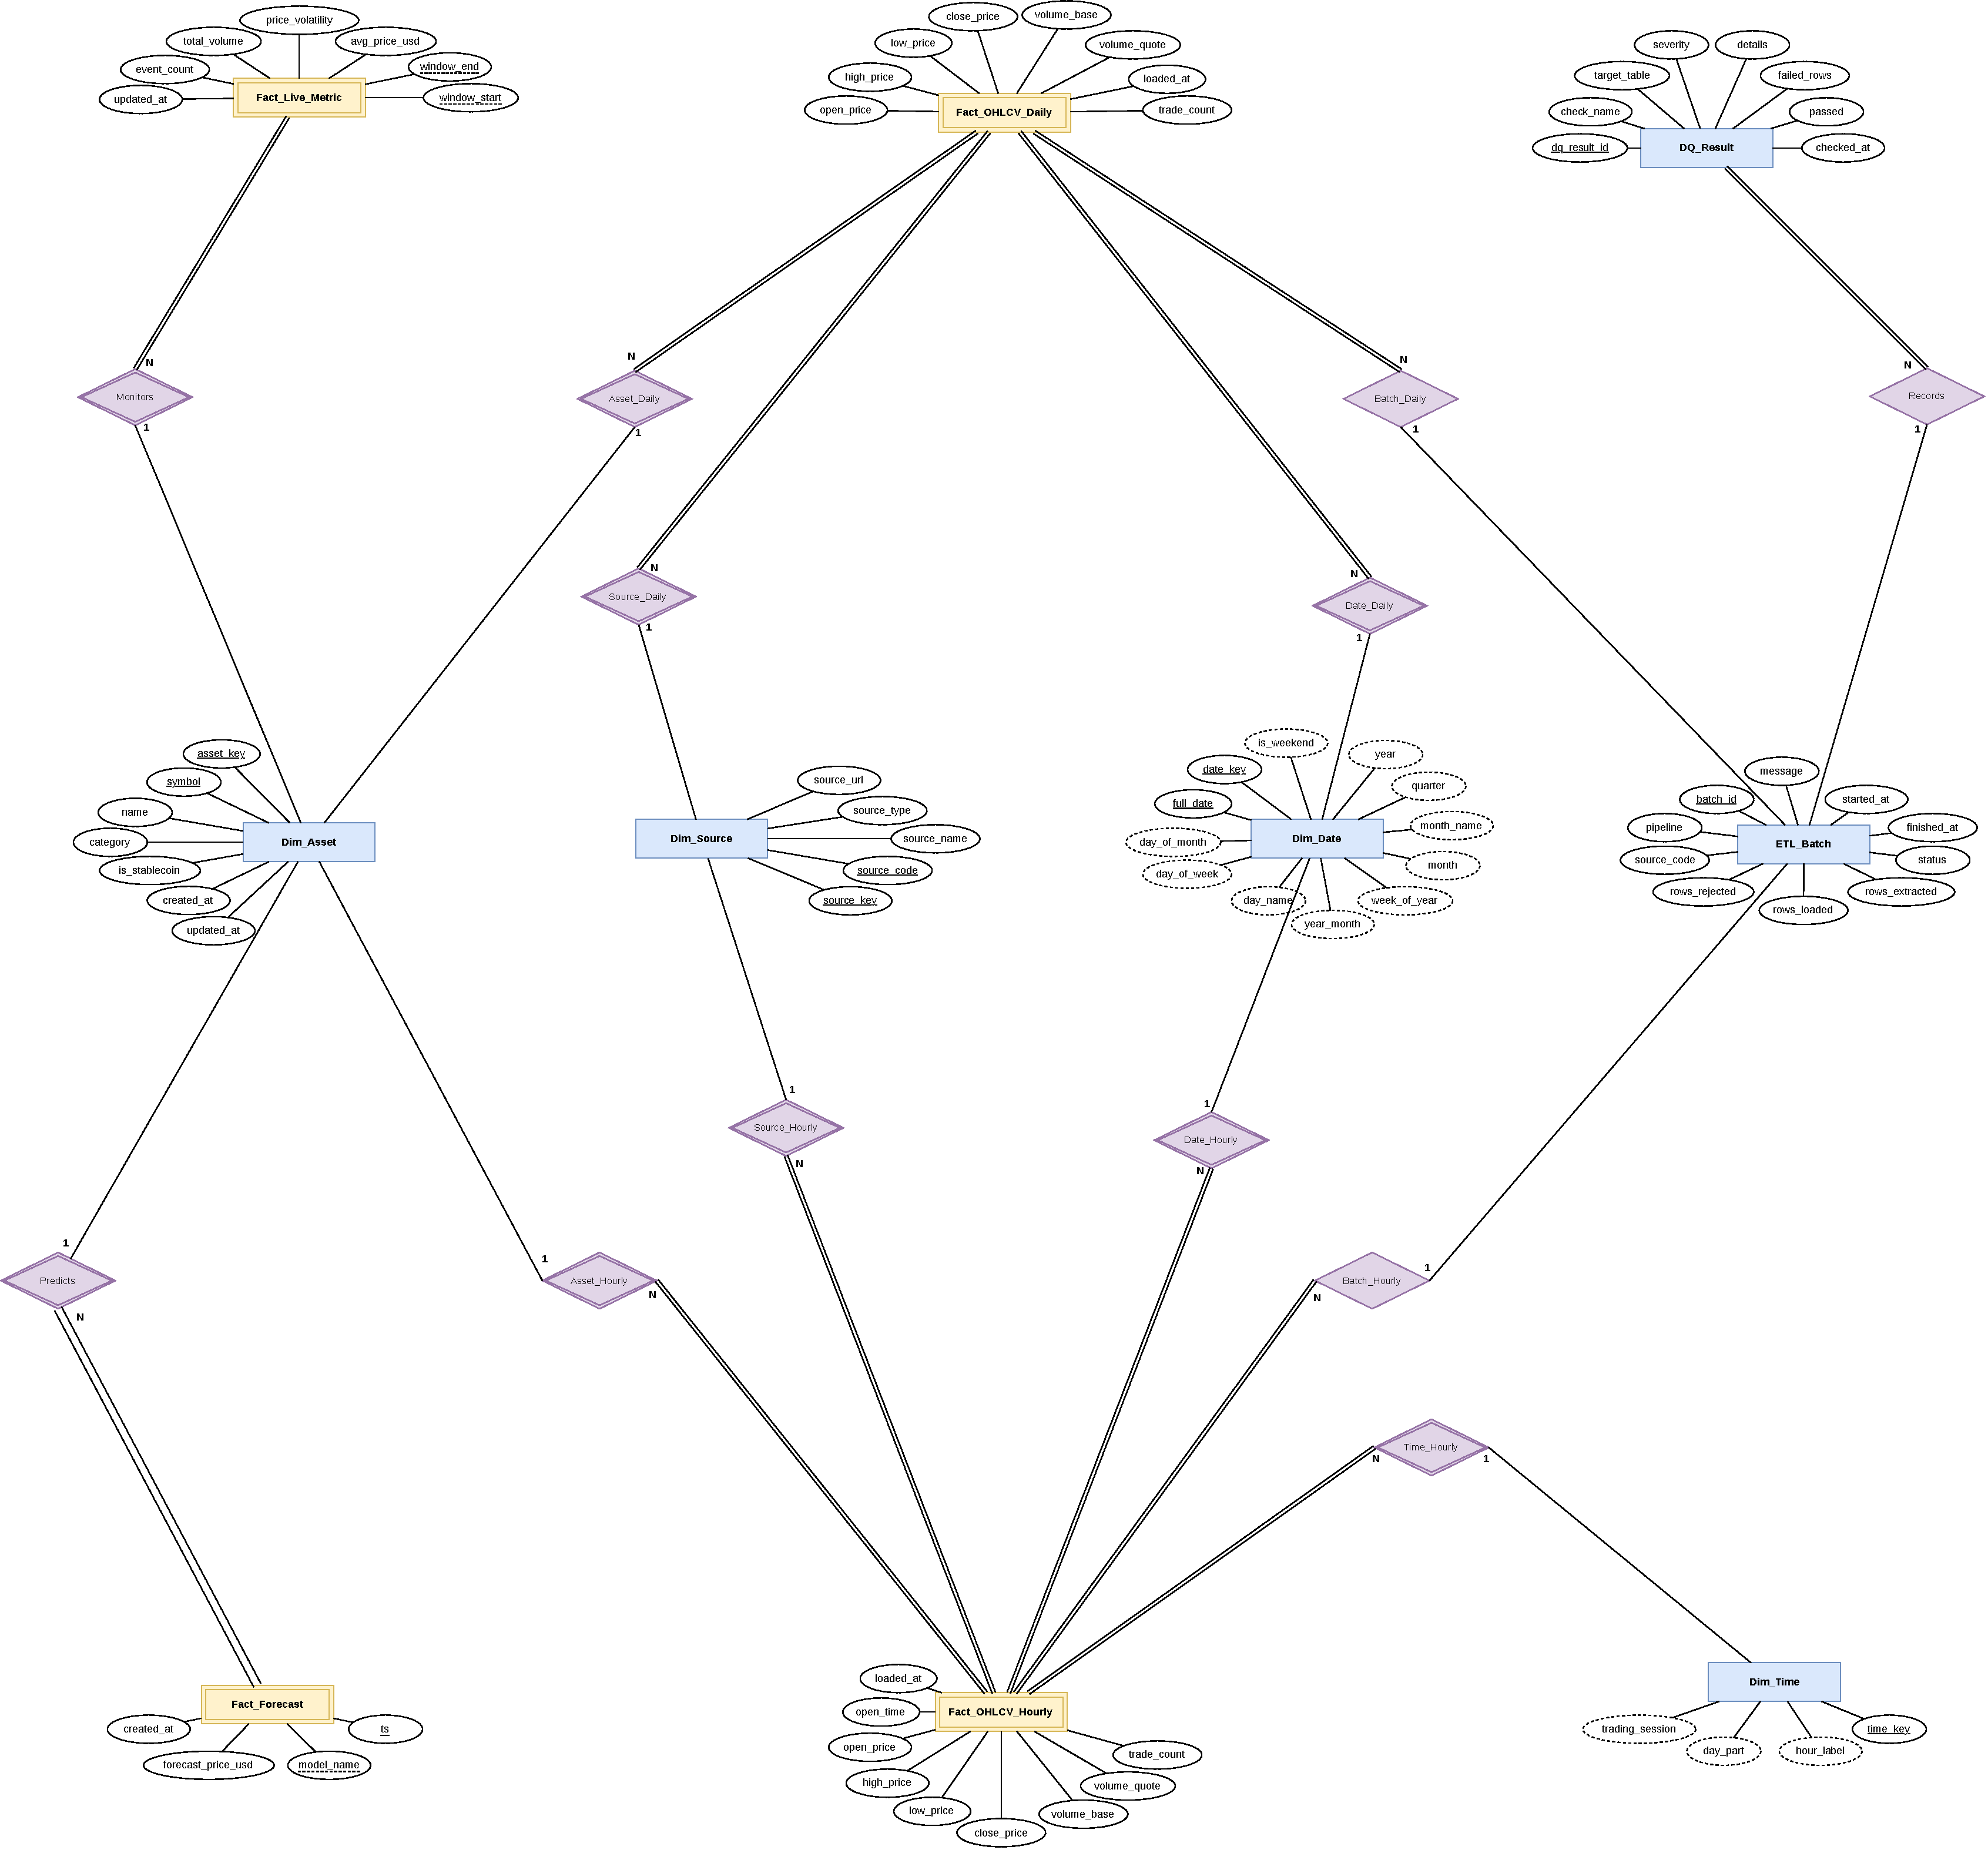
\includegraphics[width=\linewidth,height=0.42\textheight,keepaspectratio]{figures/eerd.pdf}
\caption{EERD của kho dữ liệu}\label{fig:eerd}
\end{figure}

\begin{figure}[H]
\centering
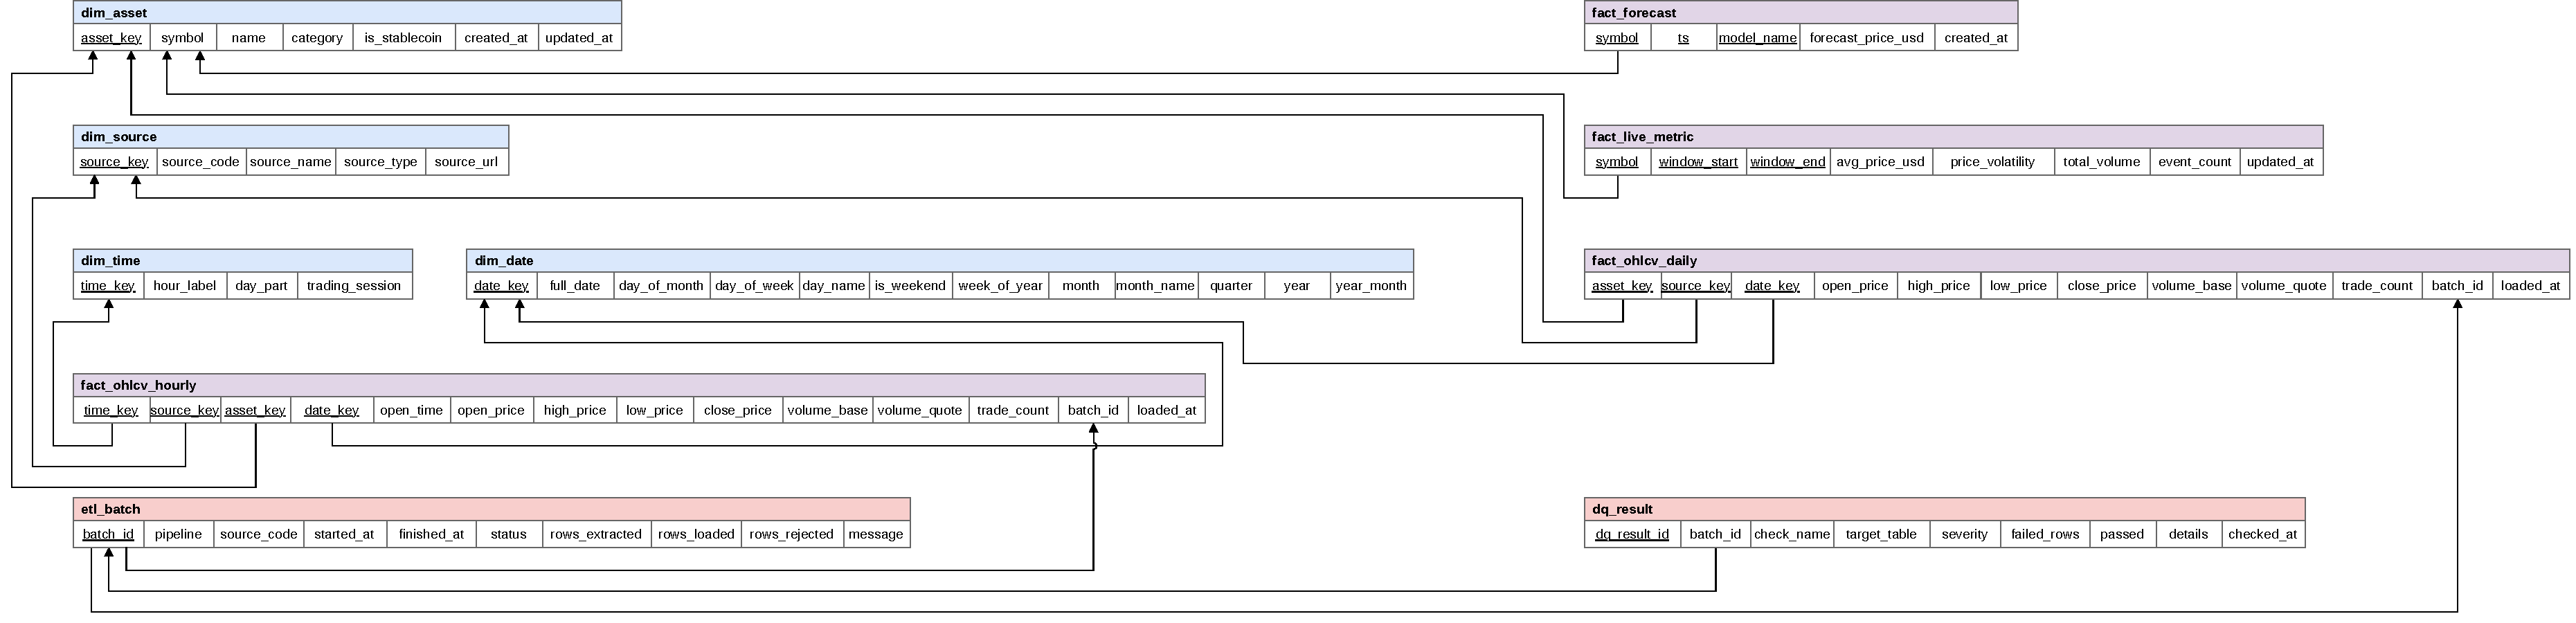
\includegraphics[width=\linewidth,height=0.42\textheight,keepaspectratio]{figures/relational.pdf}
\caption{Lược đồ quan hệ}\label{fig:rel}
\end{figure}

\subsection{Các schema}
\begin{table}[H]
\centering\small
\begin{tabularx}{\linewidth}{lX}
\toprule
\textbf{Schema} & \textbf{Vai trò} \\
\midrule
\code{staging} & Nến vừa tải, đã ép kiểu, chưa kiểm tra \\
\code{dw} & Dimension và fact đã làm sạch \\
\code{mart} & View và materialized view tổng hợp cho phân tích, dashboard \\
\code{meta} & Nhật ký mỗi lần nạp, kết quả từng rule, file nguồn đã nạp \\
\code{ml} & Sổ dự báo, đánh giá mô hình, theo dõi drift \\
\bottomrule
\end{tabularx}
\end{table}

% ---------------------------------------------------------------- 5
\section{Quy trình ETL}

\subsection{Extract}
Script tải file ZIP nến \code{1d} và \code{1h} từ Binance Public Data, kiểm tra SHA-256 với file
\code{.CHECKSUM} đi kèm, rồi lưu cache trên đĩa. Bảng \code{meta.loaded\_archive} ghi các file
đã nạp; file đã nạp sẽ được bỏ qua ở lần chạy sau.

\subsection{Staging}
Dữ liệu giải nén được ép kiểu và \code{COPY} vào \code{staging.stg\_ohlcv}. Staging là bảng thật,
giữ được dữ liệu để kiểm tra lại khi lần nạp lỗi.

\subsection{Kiểm tra chất lượng}
Có 7 rule loại dòng và 5 rule cảnh báo. Nếu hơn 5\% số dòng của một lần nạp bị loại,
cả lần nạp bị hủy, vì khi đó lỗi thường nằm ở nguồn hoặc ở parser chứ không ở từng dòng.

\begin{table}[H]
\centering\small
\begin{tabularx}{\linewidth}{llX}
\toprule
\textbf{Rule} & \textbf{Mức} & \textbf{Kiểm tra} \\
\midrule
\code{not\_null} & Loại & Đủ mã coin, giá, khối lượng \\
\code{positive\_price} & Loại & Mọi giá $> 0$ \\
\code{ohlc\_consistency} & Loại & $high \ge \max(open, close)$, $low \le \min(open, close)$ \\
\code{non\_negative\_volume} & Loại & Khối lượng, số giao dịch $\ge 0$ \\
\code{interval\_alignment} & Loại & Nến bắt đầu đúng mốc ngày/giờ UTC \\
\code{known\_source} & Loại & Nguồn có trong \code{dim\_source} \\
\code{date\_in\_calendar} & Loại & Ngày có trong \code{dim\_date} \\
\midrule
\code{duplicate\_grain} & Cảnh báo & Nến trùng grain; giữ bản mới nhất \\
\code{zero\_volume} & Cảnh báo & Nến không có giao dịch \\
\code{continuity\_gaps} & Cảnh báo & Thiếu nến giữa hai nến \\
\code{freshness} & Cảnh báo & Nến mới nhất cũ hơn 2 ngày \\
\code{daily\_hourly\_reconciliation} & Cảnh báo & Khối lượng ngày lệch $>1\%$ so với tổng 24 giờ \\
\bottomrule
\end{tabularx}
\caption{Các rule chất lượng dữ liệu}
\end{table}

Rule cuối đối chiếu hai bảng fact với nhau. Cả hai bảng được nạp độc lập từ nến gốc
(không suy bảng ngày từ bảng giờ), nên sự khớp nhau là bằng chứng hai luồng nạp đúng.

\subsection{Load: upsert idempotent}
Fact được nạp bằng một câu \code{INSERT \ldots ON CONFLICT} trên khóa grain. Mệnh đề
\code{WHERE \ldots IS DISTINCT FROM} khiến dòng chỉ được cập nhật khi số đo thật sự đổi;
\code{RETURNING} cho biết chính xác những dòng nào đã thay đổi.

\begin{lstlisting}[language=psql]
insert into dw.fact_ohlcv_daily as f (asset_key, date_key, source_key, ...)
select a.asset_key, to_char(v.open_time at time zone 'UTC','YYYYMMDD')::int, ...
from stg_valid v
join dw.dim_asset  a on a.symbol = v.symbol
join dw.dim_source s on s.source_code = v.source_code
on conflict (asset_key, date_key, source_key) do update set
    open_price = excluded.open_price, ..., batch_id = excluded.batch_id
where (f.open_price, f.high_price, ...) is distinct from
      (excluded.open_price, excluded.high_price, ...)
returning asset_key, source_key;
\end{lstlisting}

Materialized view của mart được refresh trong cùng transaction với lần nạp fact, nên người
dùng không bao giờ thấy mart tính trên dữ liệu nạp dở.

\subsection{Đối soát và kiểm chứng nạp lại}
Mỗi lần nạp ghi một dòng vào \code{meta.warehouse\_load\_report}, thỏa đẳng thức
\[ staged = rejected + duplicate + accepted. \]
Nếu đẳng thức sai, có dòng bị mất không rõ lý do. Lệnh \code{prove\_archive\_reload} tính
SHA-256 trên toàn bộ nội dung bảng fact trước và sau khi nạp lại cùng archive; hai giá trị
bằng nhau chứng minh lần nạp là idempotent.

\subsection{Điều phối}
DAG Airflow \code{coinsight\_warehouse\_daily} chạy lúc 06:00 UTC mỗi ngày: tải archive của ngày
vừa đóng, kiểm tra, nạp, refresh mart. DAG \code{coinsight\_direction\_daily} chạy lúc 07:30 UTC
để tạo dự báo, train lại vào thứ Hai. Nếu sau 07:00 UTC kho chưa có ngày hôm qua, tab Data trên
dashboard báo trạng thái \emph{Behind}.

\subsection{Luồng trực tiếp}
Producer nhận nến phút đã đóng từ Binance WebSocket, dùng REST để bù nến bị lỡ khi mất kết nối,
rồi gửi vào Kafka. Spark Structured Streaming đọc Kafka, loại trùng theo \code{event\_id} với
watermark 1 ngày, ghi \code{fact\_candle\_minute\_live} và số đo cửa sổ 7 ngày. Sau khi commit,
PostgreSQL phát \code{NOTIFY}; FastAPI đẩy qua WebSocket tới giao diện. Dữ liệu trực tiếp chỉ
dùng để theo dõi thị trường hiện tại; phân tích lịch sử và mô hình chỉ dùng dữ liệu batch.

% ---------------------------------------------------------------- 6
\section{OLAP và mart}

\begin{table}[H]
\centering\small
\begin{tabularx}{\linewidth}{llX}
\toprule
\textbf{Mart} & \textbf{Phép} & \textbf{Câu hỏi trả lời} \\
\midrule
\code{v\_daily\_return} & window \code{lag} & Lợi suất, biên độ từng ngày; nền cho các mart khác \\
\code{mv\_asset\_period\_summary} & \code{ROLLUP} & Hiệu suất coin theo tháng $\rightarrow$ quý $\rightarrow$ năm $\rightarrow$ toàn kỳ \\
\code{mv\_category\_performance} & \code{CUBE} & Nhóm coin nào sinh lời, rủi ro nhất theo mọi tổ hợp năm, quý \\
\code{mv\_hourly\_activity} & \code{GROUPING SETS} & Phiên, giờ nào sôi động và biến động nhất \\
\code{v\_top\_movers} & \code{rank()} & 3 coin tăng, giảm mạnh nhất mỗi quý \\
\bottomrule
\end{tabularx}
\caption{Các mart OLAP}
\end{table}

\subsection{Roll-up và drill-down}
\code{mv\_asset\_period\_summary} gom theo \code{ROLLUP(year, quarter, month)}, tạo bốn mức: tháng,
quý, năm và toàn kỳ. Cột \code{period\_level} ghi mức của từng dòng, nên dashboard drill-down
bằng một điều kiện lọc thay vì gọi \code{GROUPING()}.

\subsection{Slice và dice}
\code{mv\_category\_performance} trả lời trực tiếp câu hỏi mở đầu. \code{CUBE} trên ba chiều tạo
$2^3 = 8$ tổ hợp tổng con; dòng tổng được gán nhãn \code{'ALL'} thay vì \code{NULL}. Stablecoin bị
loại vì giá của chúng được thiết kế để không đổi.

\begin{lstlisting}[language=psql]
select r.source_code,
  case when grouping(r.category) = 1 then 'ALL' else r.category end as category,
  d.year, d.quarter,
  grouping(r.category, d.year, d.quarter) as grouping_id,
  avg(r.daily_return)          as avg_daily_return,
  stddev_samp(r.daily_return)  as daily_volatility,
  sum(r.volume_quote)          as volume_usd
from mart.v_daily_return r
join dw.dim_date d using (date_key)
where not r.is_stablecoin
group by r.source_code, cube (r.category, d.year, d.quarter);
\end{lstlisting}

Slice một quý: \code{where year = 2026 and quarter = 3 and category <> 'ALL'}. Dice: thêm điều kiện
trên nhóm coin.

\subsection{Hoạt động theo giờ}
\code{mv\_hourly\_activity} dùng \code{GROUPING SETS} với sáu tổ hợp (coin $\times$ phiên $\times$ giờ,
coin $\times$ phiên, coin, phiên $\times$ giờ, phiên, tổng). Chỉ sáu tổ hợp cần thiết được tính,
thay vì $2^3$ của \code{CUBE}.

% ---------------------------------------------------------------- 7
\section{Hệ hỗ trợ quyết định}

\subsection{Quy trình ra quyết định}
\begin{table}[H]
\centering\small
\begin{tabularx}{\linewidth}{lX}
\toprule
\textbf{Pha (Simon)} & \textbf{Trong CoinSight} \\
\midrule
Intelligence & Mart OLAP, phát hiện bất thường (Isolation Forest, MAD) và tab Data cho biết thị trường đang ở đâu, dữ liệu có đủ tin cậy không \\
Design & Xây dựng các mô hình dự báo, so với baseline trên tập kiểm định theo thời gian \\
Choice & Chỉ công bố tín hiệu khi mô hình tốt hơn baseline; chính sách paper trade chuyển dự báo thành quyết định mô phỏng \\
\bottomrule
\end{tabularx}
\end{table}

\subsection{Dự báo hướng giá theo ngày}
Sau khi nến ngày $D$ đóng và được nạp, xác suất giá đóng ngày $D+1$ cao hơn ngày
$D$ là bao nhiêu? Áp dụng cho BTC, ETH, SOL.

Đặc trưng lấy từ \code{dw.fact\_ohlcv\_daily}: \code{return\_1d}, \code{return\_7d},
\code{range\_pct}, \code{volume\_change}; \code{hourly\_range} tính từ đủ 24 nến của
\code{dw.fact\_ohlcv\_hourly}. Nhãn chỉ hợp lệ khi ngày kế tiếp đúng là $D+1$.

Mô hình là logistic regression chung cho ba coin. 30 ngày cuối làm tập kiểm định, 30 ngày
trước đó làm tập kiểm tra, chia theo thứ tự thời gian. Baseline là tỷ lệ ngày tăng trong tập train.
Thước đo là Brier score
\[ BS = \frac{1}{N}\sum_{i=1}^{N} (p_i - y_i)^2, \]
càng thấp càng tốt.

Mô hình chỉ được công bố khi Brier thấp hơn baseline trên cả hai tập. Mọi
ứng viên (cả bị từ chối) được ghi vào \code{meta.model\_evaluation}; mô hình được chấp nhận vào
\code{dim\_model}; dự báo vào \code{fact\_direction\_prediction}. Khi không có mô hình đạt, giao
diện ghi \emph{``Model below baseline. Signal withheld.''} thay vì hiển thị một con số không đáng tin.

\subsection{Dự báo giá đóng cửa theo ngày bằng quantile}
Mở rộng bài toán trên, nhóm dự báo log-return ngày kế tiếp
$y_d = \ln(close_{d+1}/close_d)$ từ 90 nến ngày gần nhất. Mỗi nến có 25 đặc trưng (lợi suất,
biên độ, bóng nến, khối lượng, momentum và độ biến động 7--90 ngày, ngày trong tuần). Phiên bản
\code{daily-return-v2} ghép đặc trưng của BTC, ETH, SOL theo ngày UTC, tạo đầu vào
$90 \times 75$ cho GRU/LSTM.

GRU và LSTM dự báo ba quantile $q_{10}, q_{50}, q_{90}$ bằng pinball loss:
\[ L = \tfrac{1}{3}\sum_{\tau \in \{0.1, 0.5, 0.9\}} \rho_\tau(y - \hat{y}_\tau)
  + \lambda \cdot L_{rank}. \]
Quy tắc tin cậy: $q_{10} > 0$ là \emph{chắc tăng}, $q_{90} < 0$ là \emph{chắc giảm}, khoảng
cắt qua 0 là \emph{không chắc}. Tập kiểm tra chỉ được dùng một lần; sau khi dùng, hệ thống đánh
dấu \code{TEST\_CONSUMED} để không chỉnh tham số theo kết quả kiểm tra.

\TODO{Dương: điền bảng kết quả test của GRU/LSTM/XGBoost (directional accuracy, coverage q10--q90, so với majority baseline).}

\subsection{Chính sách paper trade}
Chính sách \code{daily-quantile v1} chuyển dự báo thành quyết định mô phỏng: chỉ mua/bán spot (không
bán khống), giao dịch khi tín hiệu vượt ngưỡng 5\%, mỗi lệnh tối đa 8\% danh mục, dừng khi danh mục
sụt quá 25\% hoặc thị trường sụt quá 35\%, giá cũ hơn 300 giây thì không giao dịch. Chính sách chỉ
chạy mô phỏng, chưa có mô hình phí và chưa được duyệt cho giao dịch thật.

\subsection{Dự báo theo giờ: một kết quả âm có cơ sở}
Nhóm cũng thử dự báo lợi suất giờ kế tiếp của BTC. Thước đo là Relative MAE: MAE của mô hình chia
MAE khi luôn dự báo 0. Kế hoạch chia dữ liệu, thước đo và mục tiêu 0,97 được khóa trước khi train.

\begin{table}[H]
\centering\small
\begin{tabular}{llrr}
\toprule
\textbf{Mô hình} & \textbf{Giai đoạn} & \textbf{Số giờ} & \textbf{Relative MAE} \\
\midrule
Ensemble 2 $\times$ CatBoost & 7--12/2025 (tập chọn) & 4.416 & 0,9929 \\
CatBoost & 7--12/2025 & 4.416 & 0,9940 \\
XGBoost & 7--12/2025 & 4.416 & 0,9957 \\
TCN, LSTM & 7--12/2025 & 4.416 & 0,9974--0,9987 \\
Bản đóng băng đang phục vụ & 1--10/2026 & 6.984 & 0,9970 \\
\bottomrule
\end{tabular}
\caption{Dự báo lợi suất BTC theo giờ}
\end{table}

Mục tiêu 0,97 không đạt. Trên năm 2026, độ chính xác hướng là 52,96\%. Kết luận: lợi suất giờ gần
như không dự báo được từ dữ liệu thị trường công khai. Mô hình được giữ như một công cụ tham khảo
có ghi rõ giới hạn, không phải tín hiệu giao dịch. Khoảng tin cậy 95\% của ensemble (0,9900--0,9961)
tính bằng circular block bootstrap, khối 168 giờ, 2.000 lần lấy mẫu.

\subsection{Phát hiện bất thường}
Isolation Forest train trên 2023--2024, hiệu chỉnh trên 2025, đánh dấu 78 trên 6.984 giờ năm 2026
(1,12\%), so với 101 giờ (1,45\%) của quy tắc median/MAD. Không có nhãn bất thường nên đây là tỷ lệ
cảnh báo, không phải precision hay recall.

\subsection{Giao diện hỏi đáp}
Người dùng hỏi bằng ngôn ngữ tự nhiên, ví dụ ``Quý 3 nhóm coin nào tăng mạnh nhất?''. Hai agent
LangGraph trả lời: agent phân tích (thị trường, mart, dự báo) và agent vận hành (dữ liệu thiếu, nạp
lỗi, drift mô hình). Agent chỉ đọc kho qua role \code{coinsight\_observer} không có quyền ghi.
Mọi con số trong câu trả lời phải xuất hiện trong kết quả công cụ; câu trả lời có số không khớp
bị chặn trước khi tới người dùng.

% ---------------------------------------------------------------- 8
\section{Hiện thực và kết quả}

\subsection{Số liệu kho}
\begin{table}[H]
\centering\small
\begin{tabular}{lr}
\toprule
\textbf{Chỉ số (ngày 25/10/2026)} & \textbf{Giá trị} \\
\midrule
Số coin trong \code{dim\_asset} & 20 \\
Nến ngày & 6.238 (không thiếu) \\
Nến giờ & 175.809 \\
Nến giờ thiếu & 81 (BTC 31, ETH 31, SOL 19) \\
Lần nạp gần nhất & 500 dòng nhận, 0 dòng loại \\
Kiểm chứng nạp lại & checksum fact trước = sau \\
\bottomrule
\end{tabular}
\caption{Số liệu kho dữ liệu}
\end{table}

81 nến giờ thiếu được rule \code{continuity\_gaps} ghi nhận dưới dạng cảnh báo, không chặn lần nạp.
\TODO{xác nhận nguyên nhân: archive Binance không có giờ đó hay lỗi nạp}

\subsection{Đánh giá agent hỏi đáp}
Agent được đánh giá trên một kho giả lập với 10 tình huống dữ liệu (thiếu nến, nạp lỗi, drift,
\ldots), chia train/validation/test. Tập test chỉ chạy một lần cho mỗi phiên bản agent.

\begin{table}[H]
\centering\small
\begin{tabular}{lr}
\toprule
\textbf{Chỉ số trên tập test (14 câu, Claude Haiku 4.5)} & \textbf{Kết quả} \\
\midrule
Điểm tổng & 92,9\% \\
Chọn đúng công cụ & 100\% \\
Con số không có nguồn & 1,1\% \\
Chống prompt injection & 100\% \\
Từ chối yêu cầu ghi dữ liệu / tư vấn đầu tư & 50\% \\
\bottomrule
\end{tabular}
\caption{Đánh giá agent}
\end{table}

Tập test nhỏ (14 câu) nên khoảng bất định lớn; tỷ lệ từ chối 50\% là điểm yếu cần sửa.

\subsection{Giao diện}
Dashboard gồm danh sách coin, biểu đồ nến phút trực tiếp, biểu đồ giá đóng ngày, tab Data (số
dòng, độ phủ, nến thiếu, trạng thái nạp), tín hiệu dự báo kèm Brier và lineage, và khung hỏi đáp.
\TODO{chèn 2--3 ảnh chụp màn hình dashboard vào figures/}

% ---------------------------------------------------------------- 9
\section{Hạn chế và hướng phát triển}

Hạn chế lớn nhất nằm ở độ phủ. \code{dim\_asset} có 20 coin nhưng ETL batch mới nạp đủ lịch sử
cho 6 coin; 14 coin còn lại chỉ có dữ liệu gần đây. So sánh nhóm coin qua nhiều năm vì vậy
chỉ đáng tin với các nhóm có đủ coin trong 6 coin đó. Việc cần làm tiếp là backfill 14 coin này từ archive tháng.

\code{fact\_live\_metric} tham chiếu \code{dim\_asset} bằng \code{symbol} thay vì \code{asset\_key}.
Lỗi này nhỏ nhưng đi ngược thiết kế khóa thay thế ở các bảng còn lại; nhóm sẽ thêm cột
\code{asset\_key} và chuyển dần truy vấn sang.

\code{dim\_asset} dùng SCD loại 1, nên khi một coin đổi nhóm, mọi số liệu cũ cũng chuyển theo
nhóm mới. Với 20 coin và câu hỏi hiện tại thì chấp nhận được. Nếu cần phân tích theo nhóm tại
thời điểm đó, \code{category} phải chuyển sang SCD loại 2.

Ở mô hình ngày, nhóm đã chọn ứng viên nhiều lần dựa trên điểm tập kiểm tra, nên tập này không
còn độc lập. Mô hình giờ đã làm đúng (khóa kế hoạch trước, tập test dùng một lần); mô hình ngày
cần làm lại theo cách đó.

Agent hỏi đáp mới được đánh giá trên 14 câu test, và chỉ từ chối được một nửa số yêu cầu ghi dữ
liệu hoặc xin lời khuyên đầu tư. Cần thêm câu test và sửa prompt từ chối.

% ---------------------------------------------------------------- 10
\section{Phân công}

\begin{table}[H]
\centering\small
\begin{tabularx}{\linewidth}{lX}
\toprule
\textbf{Thành viên} & \textbf{Công việc} \\
\midrule
Hà Bảo Nhi & Thiết kế kho (bus matrix, grain, dimension, EERD, lược đồ quan hệ); extract Binance; staging; 12 rule chất lượng; upsert; mart OLAP \code{ROLLUP}/\code{CUBE}/\code{GROUPING SETS}; DAG Airflow nạp kho \\
Lê Chí Đại & Luồng trực tiếp Kafka/Spark, \code{fact\_live\_metric}, \code{fact\_candle\_minute\_live}; FastAPI; dashboard React; agent hỏi đáp và đánh giá; quan sát hệ thống; triển khai \\
Đào Quang Dương & Thiết kế bài toán dự báo; pipeline đặc trưng, snapshot, chia dữ liệu theo thời gian; XGBoost, GRU, LSTM quantile; đánh giá so với baseline; chính sách paper trade; \code{fact\_direction\_prediction} \\
\bottomrule
\end{tabularx}
\end{table}

% ---------------------------------------------------------------- 11
\section{Kết luận}
CoinSight xây dựng một kho dữ liệu galaxy schema cho nến giá crypto, với ETL kiểm tra chất lượng,
nạp lại idempotent và truy vết được tới file nguồn. Các mart OLAP trả lời trực tiếp câu hỏi phân
tích theo quý, nhóm coin và phiên giao dịch. DSS dựa trên kho đưa ra xác suất hướng giá, nhưng chỉ
công bố khi tốt hơn baseline. Kết quả nhóm thu được là lợi suất ngắn hạn gần như không dự báo
được từ giá và khối lượng. Việc tiếp theo là backfill 14 coin còn thiếu và làm lại đánh giá
mô hình ngày với một tập test chỉ dùng một lần.

\begin{thebibliography}{9}
\bibitem{inmon} W. H. Inmon, \emph{Building the Data Warehouse}, 4th ed. Wiley, 2005.
\bibitem{kimball} R. Kimball, M. Ross, \emph{The Data Warehouse Toolkit}, 3rd ed. Wiley, 2013.
\bibitem{turban} E. Turban, J. E. Aronson, T.-P. Liang, \emph{Decision Support Systems and Intelligent Systems}, 7th ed. Prentice-Hall, 2005.
\bibitem{sharda} R. Sharda, D. Delen, E. Turban, \emph{Analytics, Data Science, \& Artificial Intelligence: Systems for Decision Support}, 7th ed. Pearson, 2020.
\bibitem{han} J. Han, M. Kamber, J. Pei, \emph{Data Mining: Concepts and Techniques}, 3rd ed. Morgan Kaufmann, 2012.
\bibitem{binance} Binance, \emph{Binance Public Data}, \url{https://data.binance.vision}.
\end{thebibliography}

\end{document}
